\section{Unsupervised text classification}
\label{uns-class}

\paragraph{Text classification}
The problem of associating texts, so documents, to classes, represented by labels.
Classes may be a partition of the document space, or they can overlap.
The approaches to solve the problem are basically two, pre-trained models, 
so supervised, or based only on documents, so unsupervised.

Depending on the number of classes and how the cover the document space, we define 
four tasks
\begin{center}
    \begin{tabular}{c | c |c}
            & 2 classes & Many classes\\
            \hline
            Disjoint classes & Binary classification & Multi-class classification\\
            \hline
            Overlapping classes & Soft binary classification & Multi-label classification\\
    \end{tabular}
\end{center}

Note that ranking can be seen as soft binary classification.

\subsection{Clustering}

\paragraph{Goal}
Clustering is the problem of grouping objects in clusters, in particular
given a distance metric, 
we want to minimize the distance within a cluster and maximize the one
between different clusters.

\paragraph{Parameters}
Choosing the right number of clusters is pretty difficult, a high number 
leads to consistency inside clusters, but poor aggregation, while a low number 
increases aggregation but reduce quality of the single clusters.

\paragraph{Types of clustering}
There are many approaches to clustering, one could for instance 
consider flat or hierarchical clustering, in the first one there is no structure, where 
in the second clusters might contain other clusters. 
There is also a difference in cluster assignment, one could assign in an hard or soft way.

\subsubsection{Support to document retrieval}

\paragraph{Terminological analysis}
After computing a clustering of documents we could analyze terminology 
of documents of the same cluster to extract relevant terms, this 
information can then be used for query expansion.

\paragraph{Cluster pruning}
By selecting representative documents for clusters, we can compare a query 
only to those documents. After finding a match all the documents in the cluster 
are returned.

\subsubsection{Evaluation}
Given $\Omega = \{ \omega_1, \dots, \omega_n\}$ the set of clusters 
and $\mathbb{C} = \{ c_1, \dots, c_n\}$ the set of classes, we can evaluate 
the clustering by focusing on pairs of documents.

Let's consider the pair $(x_i, x_j)$, we ask ourselves if 
$$\exists \omega_k : (x_i, x_j) \in \omega_k\;\;\exists c_z : (x_i, x_j) \in c_z$$
They represent the clustering and the real world scenario.
If the two are true, we find a true positive, if they are both false a true negative.
In the case the first one is true and the second is not, we have a false positive, 
a false negative otherwise.

We can observe that choosing a small number of clusters leads to a large 
quantity of false positives, while a fine grain partition, i.e. a high number 
of clusters, produces a high number og false negatives.

\paragraph{Measures}
We can use some measures of quality in clustering, 
for instance 
$$\mathit{Rand} = \frac{\mathit{TP} + \mathit{TN}}{\mathit{TP} + \mathit{TN} + \mathit{FP} + \mathit{FN}}$$
but also \emph{Purity} and \emph{Normalized Mutual Information}.

\subsection{K-means}
This approach starts with $k$ random centroids and assign each data point 
to the closets one. We then recompute the centroids with the current clusters 
and repeat the first point until termination.

The termination criterion could be a fixed number of iterations, no change 
in documents assignments or \emph{RSS} measure below a threshold:
$$\mathit{RSS} = \sum_{k=1}^K\sum_{\vec{x} \in \omega_k}|\vec{x} - \vec{\mu}(\omega_k)|^2$$
where the measure is the sum of the distances between a point and it's centroid squared.
Note that at each iteration the \emph{RSS} decrease.

Two issues of this approach is that the initial position of clusters
changes the results a lot, and also, the $k$ parameter is crucial to the 
algorithm.
A good value for $k$ is $K = \min_K(\min(\mathit{RSS}_K) + \lambda K )$

\subsection{Model-based clustering}
A k-means generalization is obtained by interpreting the centroids as a model 
that generates data. A centroid with some added noise can generate a document.

\paragraph{Idea}
Instead of generating classes, we start from the points, 
we assume that they were generated with a generative model 
and we estimate the latent model parameters.

\paragraph{Latent parameters}
$\Theta = \{ \vec{\mu}_1, \dots, \vec{\mu}_n\}$ are the centroids 
to be found by k-means.

$L(D | \Theta)$ is the log-likelihood that the data $D$ wa generated by $\Theta$, 
this is the objective function, so $\Theta$ becomes:
$$\Theta = \max_{\Theta} L(D|\Theta) = \max_\Theta\sum_{n=1}^N \log P(d_n | \Theta)$$

That means maximizing the sum of probabilities that documents are generated by 
the model. We are in a soft clustering scenario, as we are 
basically dealing with probabilities
as cluster assignments.

\subsubsection{Expectation Maximization algorithm}
This is an iterative algorithm that maximizes $L(D|\Theta)$, but can also be 
used to find latent models in a variety of applications.

Let's consider a multivariate Bernoulli distribution for data, 
so all documents are binary vectors, 
we want to estimate the probability that a given document is assigned to a
specific cluster given the models parameters.
$$P(d | w_k; \Theta) = \prod_{t_m \in d}q_{mk} 
\cdot \prod_{t_m \notin d}(1-q_{mk})\;\;\;\Theta_k = (\alpha_k, q_{1k}, \dots, q_{Mk})$$
where $q_{mk} = P(U_m =1 | \omega _k)$ is the probability that a document from the cluster 
$\omega_k$ contains the term $t_m$.

$\alpha_k$ si the prior of the cluster $k$, so the probability that of a document 
to be in that cluster, not having any information about it.

\paragraph{Process}
We start by generating a document by picking a cluster $w_k$ with probability 
$\alpha_k$, generating terms with probability $q_{mk}$. 

We need to estimate the two parameters, and we do that iteratively similarly to k-means.
The iteration is composed by two steps, \emph{Maximization} and \emph{Expectation}.

\paragraph{Maximization step}
The goal here is to estimate the parameters of the model, so the prior and the 
terms probability given the cluster:
$$q_{mk} = \frac{\sum_{n=1}^N r_{nk}I(t_m \in d_m)}{\sum_{n=1}^N r_{nk}}
\;\;\; \alpha_k = \frac{\sum_{n=1}^N r_{nk}}{N}$$
where $I$ can be one or zero wether the term appears or not in the 
document, and $r_{nk}$ is the soft assignment of the document $n$ to the 
cluster $k$.


\paragraph{Expectation step}
We now estimate the probability of each term to be assigned to a cluster.
$$r_{nk} = \frac{\alpha_k(\prod_{t_m \in d_n}q_{mk})(\prod_{t_m \notin d_n}(1-q_{mk}))}
{\sum_{k=1}^K\alpha_k(\prod_{t_m \in d_n}q_{mk})(\prod_{t_m \notin d_n}(1-q_{mk}))}$$
this is basically, for each cluster, the prior, multiplied by the product of $q_{mk}$ or $1- q_{mk}$ for each 
term in the document
computed before, 
normalized by the same quantity over all the clusters.

\paragraph{Why do EM works?}
The main idea of the algorithm is to push documents that contains the same 
words in the same cluster. Basically if two words appears in a document 
they should have a high probability of being assigned to the same cluster, 
so they have the same $q_{mk}$. This leads to assigning documents with the 
same words in the same clusters.

\subsection{Affinity propagation clustering}

\paragraph{Input}
The input is a similarly matrix, for instance $s(i,j) = - ||\vec{i} - \vec{j}||^2$.
There are also some special values for the diagonal of the matrix, 
where larger values are more likely to be chosen as exemplars for 
clusters.

\paragraph{Idea}
Documents exchange messages to decide exemplars and clusters assignments.
This approach is similar to \emph{page rank with authorities} \footnote{\url{https://nlp.stanford.edu/IR-book/html/htmledition/hubs-and-authorities-1.html}}. 

\paragraph{Responsibility messages}
A message $r(i,k)$ that denotes how well $k$ is an exemplar for $i$.
An example can be
$$r(i, k) = s(i, k) - \max_{k^\prime s.t.k^\prime \neq k} \{ a(i, k^\prime) + s(i, k^\prime)\}$$
basically we take the similarity of a pair of nodes and subtract the maximum 
similarity for any other document. This value will be zero for the most similar 
document, and negative for all other, as the quantity $a(i, k^\prime)$ is initially zero.

\paragraph{Availability}
This message $a(i, k)$ represent how appropriate is for $i$ to choose 
$k$ as exemplar.
$$a(i, k) = \min \bigg\{ 0, r(k, k) + \sum_{i^\prime s.t.i^\prime \notin \{i, k\}} \max\{0, r(i^\prime, k)\}\bigg\}$$

\paragraph{Self availability}
The availability measure given the same document as argument, is 
$$a(k, k) = \sum_{i^\prime s.t.i^\prime \neq k} \max\{0, r(i^\prime, k)\}$$

\paragraph{Process}
At first, documents are connected by similarity, then we recompute the availability 
with respect to the responsibility and vice versa. This leads to making documents 
connections stronger and stronger and to the election of an exemplar for clusters.
After some iterations convergence is reached.

\subsection{Hierarchical clustering}
This approach produces a hierarchy of clusters. It does not need the number of clusters 
but a criterion of optimal cluster selection. Most of this algorithms are deterministic.

\paragraph{Process}
Staring from a similarity matrix for the documents, we start taking the pair 
of documents with maximum similarity and group them in the same cluster. 
An idea is to have documents as nodes, and to add a cluster node connected 
to the two most similar documents.

The next step is to delete the rows and columns of the two selected documents, 
as they are already assigned, but, we add a new row and column 
for the cluster node.
The similarity value between a document and a cluster is the minimum similarity 
in that cluster for the considered document, but many strategies can be applied.

After rebuilding the table, we continue with the initial step, 
note that if a cluster and document are selected as most similar items, 
we are adding a cluster connected to them, ergo we are considering the cluster 
obtained in the first step, as a sub-cluster for the last one.

The last step is to select the number of clusters.
The previous logic created tree, as we grouped documents and clusters by adding 
nodes connected to them.
We can choose a threshold for the intra-cluster similarity, or select a certain 
number of clusters, or considering the maximum jump in similarity in the obtained cluster
tree and cut off the tree there. By cutting off the tree, we take the lower part, so 
the one with the leaves.

\begin{figure}[h]
    \centering
    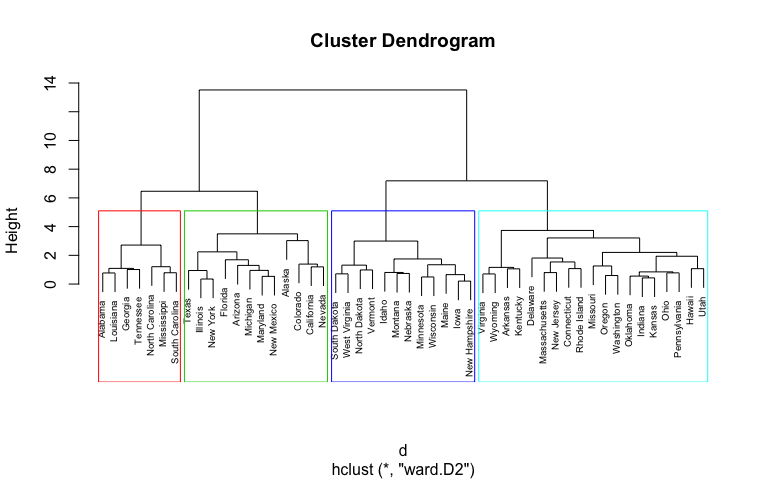
\includegraphics[width=0.8\textwidth]{images/hierarchical-clustering.png}
    \caption{Hierarchical clustering example with 4 clusters}
\end{figure}

\paragraph{Top-down clustering}
This approach starts from a cluster containing all the documents, and
recursively splits it keeping track of the parent of each document. 
The process stops when a threshold of intra-cluster similarity is obtained 
or when there's a cluster for each document.
This approach is the opposite of the bottom up tree creation.
